\documentclass[12pt]{article}

%Required packages
\usepackage[utf8]{inputenc}
\usepackage{apacite}
\usepackage{caption} 
\usepackage{setspace}
\usepackage{amsmath}
\usepackage{graphicx}
\usepackage[textwidth=160mm, textheight=210mm, hmarginratio=1:1]{geometry}


%Prerequisite statements
\DeclareCaptionLabelSeparator*{spaced}{\\[2ex]} %Declare the caption and title seperator spacing
\captionsetup[table]{,textfont=it,format=plain,justification=justified,
  singlelinecheck=false,labelsep=spaced,skip=2ex} %Setting up caption for table titles
 \captionsetup[figure]{,textfont=it,format=plain,justification=justified,
  singlelinecheck=false,labelsep=spaced,skip=2ex} %Setting up caption for figure titles
\captionsetup{labelfont={bf}} %Bold label font for tables
\onehalfspacing %Document line spacing
\pagestyle{myheadings} %Heading style
\graphicspath{ {./figures/} } %Defining image path

\begin{document}

%Title page 
\begin{titlepage}
\begin{center}
\LARGE{\textbf{The Realtime Assessment of Mental Workload by Means of Multiple Bio-Signals}}\\
\vspace*{2\baselineskip}
\Large{\textbf{Master thesis Report}}\\
Methodology and Statistics for the Behavioral, Biomedical and Social Sciences\\
\vspace*{1\baselineskip}
Utrecht University\\
\vspace*{4\baselineskip}
{Bart-Jan Boverhof, 6000142}\\
\vspace*{1\baselineskip}
{\textbf{Thesis Supervisor}}\\
Prof.dr.ir. B.P. Veldkamp\\
\vspace*{1\baselineskip}
{\textbf{Date}}\\
January 11, 2020\\
\vspace*{1\baselineskip}
\end{center}
\end{titlepage}

%Introduction section
\section{Introduction}
The topic of mental workload is a widely studied 
phenomenon across a variety of different fields, amongst others the field of ergonomics \cite{young2015state}, human factors \cite{pretorius2007development} and neurosciences \cite{shuggi2017mental}. A commonly utilized definition for mental workload, hereafter referred to as simply "workload", is the demand placed upon individuals whilst they carry out a particular task. As pointed out by \citeA{de1996measurement}, the aforementioned definition is too simplistic, for it defines workload solely as an external phenomenon. Workload is, however, a person-specific construct, for the amount of perceived workload ushered by a given task may differ across individuals \cite{de1996measurement}. Hence, when referring to workload throughout this research, person-specific workload is implied specifically. 

A commonly employed method for assessing workload is the well established NASA-Task Load Index questionnaire. This questionnaire inquires the respondent on the amount of perceived workload, and is constructed from six subjective sub-scales \cite{hart2006nasa}. Such an assessment is usually conducted post-experiment, which can in certain situations be deemed undesirable. Consider an experiment in which is aimed to assess workload of a pilot in flight. An evident approach towards such an experiment is that we wish to measure the degree of perceived workload during different phases of the flight. However, only after the simulation is concluded, a measurement in the form of a questionnaire can be administrated. In such a situation, utilizing a post-experiment assessment is prone to generate bias. A widely recognized bias is the observer-bias, advocating that participants in an experiment tend to overexaggerate the treatment effect when having to report it post-experiment \cite{mahtani2018catalogue}. In the light of the aforementioned example, pilots are expected to overexaggerate the degree of perceived workload when having to report it post-experiment.

An alternative approach to the assessment of workload is to collect physiological bio-signals during the experiment, and utilize these to classify workload. Examples of such bio-signals, hereafter referred to as "modalities", include techniques as electroencephalogram, eye-tracking, galvanic skin response, functional near-infrared spectroscopy etc. The advantage of such an approach is that complementary information streams, each stemming from a different modality, may all be interpreted simultaneously \cite{ramachandram2017deep}. This has the potential of yielding a rich and multifaceted classification of construct such as workload. Additionally, it is possible to train a separate model for each individual, catering towards the individual perception of workload for that specific person. This approach, however, comes at the cost of an increase in complexity. This resides in the need to construct a complex framework that inputs the data from each of the utilized modalities, and ultimately outputs a single classification outcome. 

The current research builds upon research conducted by \citeA{dolmans2020perceived}, who proposed a deep-learning approach to multi-modular classification of workload. The current research differs from this previous endeavor in that it utilizes different modalities, and hence different data. In addition, the current research investigates upon the feasibility of a real-time approach. Real-time in this sense reflects the real-time classification of workload, i.e. the classification of workload whilst the experiment takes place. Doing so enables the possibility to conduct a dynamic experiment, the state of which can be altered by responding towards the classified degree of workload at a certain moment in time. Consider a simulation with the objective of educating its participant, such as a surgical simulation for educating surgeons-in-training. The learning experience of a single session could be dramatically enhanced when the state of the experiment is catered towards the individual learning process dynamically. For example, in case it is recognized early on in the simulation that a surgeon-in-training has difficulty with a specific procedure, the remainder of the experiment can be catered towards focusing on this specific procedure. By enhancing the learning experience in this way, the effectiveness of a single simulation session can be improved dramatically, entailing a more efficient learning process.

Three different modalities are utilized in the current research. Firstly the technique of electroencephalogram, hereafter referred to as "EEG", secondly the technique of galvanic skin response, hereafter referred to as "GSR" and thirdly the technique photoplethysmography, hereafter referred to as "PPG". It is of importance to recognize that the objective of the current research is not to gain insight into the most optimal model design for each of the previously delineated modalities. The objective is rather to construct a framework with which real-time classification can be managed, and to which modalities of choice can easily be added in future research endeavors. Consequently, one of two design principles on which the architecture of the framework reclines is the principle of modularity. Modularity refers to the extent to which different modalities can freely be added and/or removed to the framework, without the necessity to re-architect and rebuild it entirely. The second design principle is the principle of generalizability, prescribing that the framework should not merely be utilizable in the context of workload, but also for the measurement of other mental constructs.

A deep-learning approach towards the construction of a real-time multi-modular framework is realized. Considering the complexity and sheer size of such a deep-neural network, an important point of attention is classification speed. The challenge in real-time classification with deep-learning is often not reaching adequate performance, but rather to attain adequate speed of classification. Deep neural networks easily constitute thousands of calculations to be made simultaneously, which is even more true for a multi-modular approach such as the current. In order for real-time classification to work, classification cannot take too long, for otherwise it is not real-time anymore and the previously delineated benefit of a real-time approach dissipates. As a consequence, multiple networks are considered and contrasted in terms of performance and ability to classify in real-time. Firstly, for each of the three modalities separately, a single-modular network is constructed. Secondly, a multi-modular network is architected. Additionally, several variations to this multi-modular framework are considered and contrasted. These variations are specified to differ in size, i.e. the amount of neurons and filters. 

The objective of the current research is to explore the circumstances in which a multi-modular approach by means of deep learning is capable of real-time classification, whilst still ensuring ample and adequate performance. Ultimately, this line of research pursues the ability to conduct a dynamic experiment for multiple people simultaneously, and of which the state can be altered in real-time. 

%Method section
\section{Methods}

\subsection{Related Work} 
The following section will provide an overview of preceding research on the most optimal network architecture for each single-modular network. Subsequently, the most feasible architecture for the multi-modular framework in its entirety will be explored, with particular attention on the data fusion strategy and a range model optimization techniques.

\subsubsection{Electroencephalogram (EEG)}
The first utilized modality is EEG, which constitutes a technique that detects electrical activity in the brain using electrodes. EEG is a commonly utilized method within the field of workload investigation. An overview of the complete literature on EEG applications with deep-learning was presented by \citeA{craik2019deep}, who reported a total of 16 \% of all available papers to cope with workload classification. With regards to these EEG applications, \citeA{craik2019deep} reported that studies mostly found deep belief networks and convolutional neural networks, hereafter referred to as "ConvNets", to perform best when classifying workload, and advice one of these approaches as a consequence.

\citeA{tabar2016novel} proposed combining a ConvNet with a Stacked auto-encoder network, hereafter referred to as "SAE". The input layer was specified to feed into a convolutional layer with the objective of learning the filters and network parameters. The output of this convolutional layer was subsequently specified to feed into the SAE part, architected to include an input layer, 6 hidden layers and an output layer. A classification accuracy of 90 \% was acquired with this network \cite{tabar2016novel}. 

Research by \citeA{schirrmeister2017deep} contrasted the performance of several ConvNets against the widely utilized baseline method for EEG classification, filter bank common spatial pattern, hereafter referred to as "FBCSP". A deep ConvNet, a shallow ConvNet, a deep-shallow hybrid ConvNet and a residual ConvNet were contrasted with an FBCSP. Both the deep and shallow ConvNets were found to reach at least similar, and in some regard better classification results as compared with the FBCSP baseline approach. Altogether, a deep ConvNet with four convolutional-max-pooling blocks was found to perform best, exhibiting an accuracy of 92.4 \% \cite{schirrmeister2017deep}.

\subsubsection{Galvanic Skin Response (GSR)}
The second utilized modality is GSR, measuring sweat gland on the hands and hereby inferring arousal. GSR activity is known to be significantly correlated with workload, as was demonstrated amongst others by \citeA{shi2007galvanic}. As a consequence, GSR poses a widely utilized modality within the field of workload detection. 

\citeA{sun2019hybrid} explored the architecture for the most suitable deep-learning approach to the classification of several emotional states by means of GSR. Several model were explored, amongst others a support vector machine, a ConvNet, a long-short-term-memory, hereafter referred to as "LSTM", network. Additionally, a hybrid model combining the ConvNet and LSTM approaches was explored. This aforementioned hybrid model was found to perform best, exhibiting an accuracy of 74\% \cite{sun2019hybrid}. 

\citeA{dolmans2020perceived} took a multi-modular approach to workload classification, and architected a variant on the previously delineated CovNet-LSTM approach for the GSR modality specifically. The performance of this model was contrasted with a network consisting solely of fully connected dense layers. Conform with findings by  \citeA{sun2019hybrid}, the hybrid model was found to perform best, displaying an accuracy of 82 \% \cite{dolmans2020perceived}. The model architecture as utilized by \citeA{dolmans2020perceived} deployed two convolutional max-pooling blocks and two LSTM layers.

\subsubsection{Photoplethysmography (PPG)}
The third modality constitutes PPG, which is a technique utilized to measure volumetric changes in blood in peripheral circulation. \citeA{zhang2018evaluating} contrasted several approaches towards workload classification, out of which PPG was found to perform among the best. As a consequence, PPG constitutes one of the most widely utilized approaches towards workload classification. 

Work by \citeA{biswas2019cornet} investigated upon a deep-learning approach towards PPG classification, with the objective to perform both bio-metric identification and obtain heart rate information. Exceptional results were attained with a deep neural network, attaining an average accuracy of 96 \% \cite{biswas2019cornet}. This performance was realized with a ConvNet-LSTM hybrid, incorporating two convolutional max-pooling blocks followed with two LSTM layers. 

\subsubsection{Fusion Strategy}  
When taking a multi-modular deep-learning approach, information streams stemming from different modalities are required to be combined, i.e. "fused", at a certain point in the network in order to ultimately result in a single classification. Fusion can be done conforming different strategies. Several strategies as proposed by \citeA{ramachandram2017deep} have been considered.

Early, or data-level, fusion constitutes an approach that fuses data sources before being fed into the network. Techniques that manage this include for example principle component analysis and factor analysis. Early fusing is usually proven to be challenging, residing in the fact that data streams stemming from different modalities often differ in their dimensionality and sampling rate. In addition, when endeavoring an early fusion approach ,the oversimplified assumption of conditional independence is made implicitly. This assumption is unrealistic in nature, for data stemming from different modalities are expected to be correlated in practice \cite{ramachandram2017deep}. 

Late, or decision-level, fusion refers to the process of aggregating the decisions of multiple networks, each architected and applied towards each modality separately. In case the data sources stemming from the various modalities are either correlated or ultimately inhibit a different dimensionality, late fusion is a much more feasible approach as contrasted with early-fusion \cite{ramachandram2017deep}.

Lastly, intermediate fusion is the most widely employed fusion strategy for multi-modular deep-learning problems. Data streams are usually fused by concatenation of the networks defined for each modality separately, followed by a higher order layer that ultimately results in a classification. This need not be a single layer, but could be multiple layers, as long as each modality ultimately feeds into the highest order output layer. The depth of the fusion, i.e. the specified number of fusion layers, can be chosen conform to the specific circumstances, posing intermediate fusion to be the most flexible and therefore the most widely adopted fusion strategy \cite{ramachandram2017deep}.

Indeed, when consulting the literature, one is forced to conclude that intermediate fusion strategies are the most prevailing for multi-modular deep neural networks. When taking such an approach, the higher order network architecture is required to be established, for which several previous endeavors will be considered.  \citeA{rastgoo2019automatic} utilize a multi-modular ConvNet approach, and fused the modalities by concatenation, followed with two LTSM layers, two dense layers and a softmax layer. A simpler approach is utilized by \citeA{han2020classification}, who utilized an intermediate fusion approach solely consisting of several fully connected dense layers, and ending with a soft-max layer. Lastly, \citeA{dolmans2020perceived} took a relatively deep intermediate fusion approach, consisting of two dense layers, two convolutional layers followed by another two dense layers.  

\subsubsection{Model Optimization}
The technique of batch normalization was originally proposed by \citeA{ioffe2015batch}, and is often a applied in deep-learning with the objective of enhancing the stability of a network. Especially ConvNets capitalize on this technique. It is beneficial to include a batch normalization layer after each convolutional layer, re-centering and re-scaling the input feeding into subsequent layers. When incorporating a batch normalization layer, it is recommended to do so before feeding into the activation function \cite{ioffe2015batch}. An increase in accuracy for EEG classification was attained by \citeA{dolmans2020perceived} and \citeA{schirrmeister2017deep} by specifying a batch normalization layer following each convolutional layer. Equally so, the best performing network for PPG data as proposed by \citeA{biswas2019cornet} included a batch normalization layer succeeding each convolutional layer. 

Pooling layers are commonly employed in ConvNets, often subceeding a convolutional layer with the purpose decreasing dimensionality. The objective of such layers are to merge similar features into one: for a more extensive elaboration see \citeA{lecun2015deep}. Both \citeA{schirrmeister2017deep} and \citeA{tabar2016novel} specified a max-pooling layer after each convolutional layer within their EEG ConvNets. The network as proposed for GSR by \citeA{sun2019hybrid} incorporated a max-pooling layer after each but one of the convolutional layers. Lastly, the network as proposed for PPG by \cite{biswas2019cornet} specified a max pooling layer after each convolutional layer. 

Hyper-parameter optimization, hereafter referred to as "HPO", is a technique that can be used to optimize hyper-parameters such as learning rate, dropout probability and momentum. Substantial advancements within the deep learning community have been attained by utilizing HPO, especially with regards to ConvNet performance \cite{bergstra2012random}. The Optuna toolbox provides a method for creating a parameter search space, from which values for the hyper-parameters can be sampled and optimization can be performed \cite{akiba2019optuna}. 

\subsection{Data}
The subsequent section will provide an overview of the utilized data. Attention is primarily placed upon the experimental setup, the description of the respondents, the utilized devices and the synchronization process. 

\subsubsection{Experimental Setup}
The experimental setting for data collection is the open-source spaceship video-game Empty Epsilon, in which respondents are required to carry out tasks on a virtual spaceship \cite{daid2016empty}. This experiment was instituted by the Brain Computer Interfaces testbed lab, hosted by the University of Twente and carried out in cooperation with Thales group Hengelo. The experiment constituted three different segments, in each of which the respondent had to carry out tasks. These tasks were constructed to evoke varying degrees of perceived workload. Each segment consisted of six small sessions lasting roughly five to ten minutes. These sessions varied in difficulty, including two easy, two intermediate and two hard sessions per segment. A schematic overview of the experimental structure is depicted as figure \ref{fig:experimental}. 

After each small session, respondents filled in the TLX questionnaire compromising six questions each, resulting in 18 filled in questionnaires per respondent. Each questionnaire inquired upon the degree to which the respondent experienced workload during the preceding session. These ratings have been utilized to label the data for network training purposes. Within each segment, the order in which the sessions were presented was randomized. The order in which the three main segments were administrated was not randomized. Between every three sessions, respondents were requested to take a short two minute break.

\begin{figure}
\caption{Experimental setup}
\bigskip
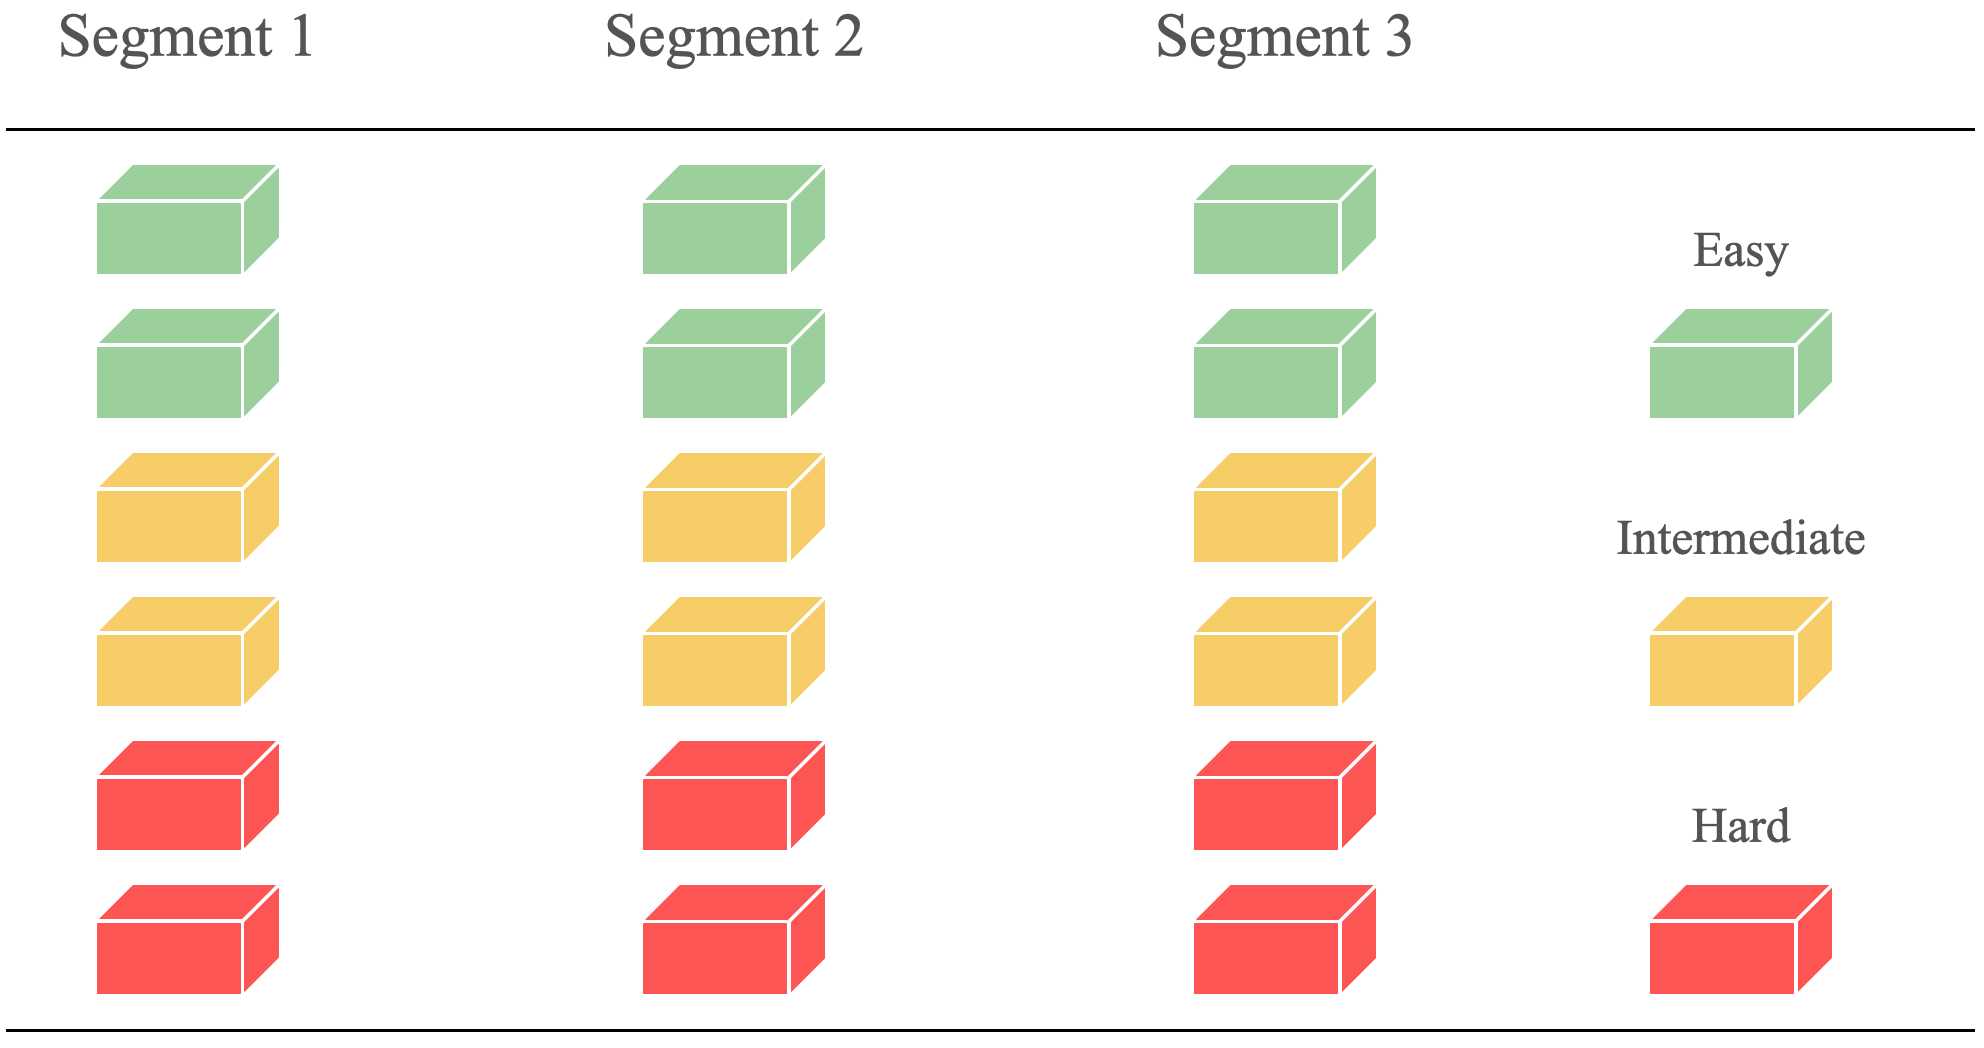
\includegraphics[scale=0.4]{experimental_setup}
\label{fig:experimental}
\end{figure}


The first segment emulated a scenario in which hostile spaceships approach the respondent's spaceship. The respondent is required to quickly react by defusing the hostiles in order to survive. The increment in difficulty caused the process of defusing hostile spaceships to become more challenging, hereby aiming to cause an increase in workload. The second segment emulated a scenario in which the respondent had to navigate their spaceship trough space, gathering as many way-points as possible. Obstacles around which the respondent had to carefully navigate and hostile spaceships the respondent had to decimate were introduced in the higher difficulty sessions. The third and final segment emulated a machine room, in which respondents had to control the power based on randomly generated requests. In the increased difficulty settings, variables that could overheat the spaceship were introduced, demanding the respondent to multi-task and aiming to increase workload.

\subsubsection{Respondents}
In total, 25 respondents have participated in the study. Currently, the data is still in the process of being collected, for which no additional descriptive statistics can be presented in the this section as of yet. The respondents are students recruited from the University of Twente. Recruitment has been conducted with Sona, which is a cloud-based participant management system. A requirements for participation was that respondents didn't have any constraints that might interfere with the utilized sensors, such as for example a pacemaker. This was assessed by means of a short demographic questionnaire prior to the experiment. Additionally, the respondents were made aware of informed consent prior to the experiment with the objective to ensure completely voluntary participation. Respondents were able to draw back from the experiment at any time. 

\subsubsection{Devices and Sampling Rate}
The Shimmer3 GSR+ sensor was used for both PPG and GSR measurements. The device is worn on the wrist, and is able to communicate both signals wirelessly. An ear-clip was utilized for measuring PPG, and converting this to estimate heart rate. Skin conductivity, or GSR, was monitored by two electrodes attached to the fingers \cite{shimmer}. EEG measurement was conducted with the Muse 2, which is a multi-sensor headband that provides feedback on brain activity \cite{muse}. The Shimmer3 GSR+ is able to read and output data signals on a sampling rate of 256 Hz, whereas the Muse 2 is able to sample at a maximum of 220 Hz. 

As was set forth in the introduction, real-time classification requires a swiftly classifying network. A higher sampling rate equals more data traveling through the network, which decelerates classification speed. As a consequence, it is necessary to input data on the minimum required sampling rate with which key features can be detected a consistent manner, for each modality separately. 

\citeA{fujita2019evaluation} investigated the required sampling rate for PPG feature detection. The extent to which important features were detected was contrasted for several sampling rates. A sampling rate of 60 Hz was found to be the absolute minimum required sampling rate for extracting all commonly utilized features in a stable manner \cite{fujita2019evaluation}. Utilizing a slightly higher sampling rate might be the safer option, however. The Shimmer3 GSR+ manufacturers recommend a sampling rate of 100 Hz for the PPG modality \cite{shimmer}. Hence, a sampling rate of 100 Hz was specified for the PPG modality. 

The required sampling rate for the GSR modality is substantially lower as compared with both PPG and EEG. In fact, the Shimmer3 GSR+ manufacturers recommend a sampling rate ranging between 0.03 and 5 Hz \cite{shimmer}. A sampling rate of 5 Hz was specified as a consequence. 

For the EEG modality, different features require a widely different sampling rate in order to be detected. Frequency bands for traditionally considered EEG features are defined on about 0.5-4 Hz for delta, and at most on about 16-24 Hz for beta. The gamma frequency band recently gained in popularity within the field of EEG however, and is defined on a frequency ranging up to 80 Hz \cite{weiergraeber2016sampling}. In order to detect a feature residing on a 80 Hz frequency band, a substantially higher sampling rate is required to record the signal without aliasing. The required sampling rate can be determined by means of the Nyquist criterion for practical EEG sampling, defined as equation \ref{eqn:nyquist},

\begin{equation}
\label{eqn:nyquist}
f_{samp} > 2.5 * f_{max}
\end{equation}
where $f_{samp}$ reflects the required sampling rate and $f_{max}$ reflects the frequency range around which the feature to be detected resides \cite{srinivasan1998estimating}. Hence, in order to be able to detect the gamma frequency band, a sampling rate of $2.5*80=200$ was specified for the EEG modality. A summary of the specified sampling rates per modality are depicted in table \ref{table:samplingrate}.

\bgroup
\def\arraystretch{1.6}%  
\begin{table}[h]
\centering
\bigskip
\caption{Sampling rate per modality}
\label{table:samplingrate}
\begin{tabular}{ll}
    & Specified sampling rate (Hz) \\ \hline
 Electroencephalogram (EEG) & 200                         \\
Galvanic Skin Response (GSR) & 5                           \\
Photoplethysmography (PPG) & 100                         \\ \hline
\end{tabular}
\end{table}
\bigskip
\egroup

\subsubsection{Synchronization}
Data streams stemming from the different modalities were required to be properly synchronized. This was accomplished by means of an application called Lab-Streaming Layer, hereafter referred to as "LSL". The data streams stemming from the different modalities were all streamed to LSL during the experiment. LSL properly synchronized these data streams, such that they are parallel time-wise. Subsequently, all data was recorded into a single file per participant \cite{kothe2018lab}.

\subsection{Framework Architecture}
As was elaborated on in the introduction, several networks have been compared in their ability to classify workload in real-time, and the performance with which this is managed. The upcoming section opens with the description of architecture of the three single-modular networks. Subsequently, the multi-modular network architecture will be elaborated on. Lastly, several variations made on this multi-modular architecture are discussed. 

\subsubsection{Single-modular Network Architectures}
The architecture of each of the single-modular networks is determined by combining insights from the literature. Each of the three networks merely utilized a single modality with which workload was classified. These networks and their architectures are depicted as figure \ref{fig:singlearchitecture}.

\begin{figure}
\caption{Three single-modular network architectures}
\bigskip
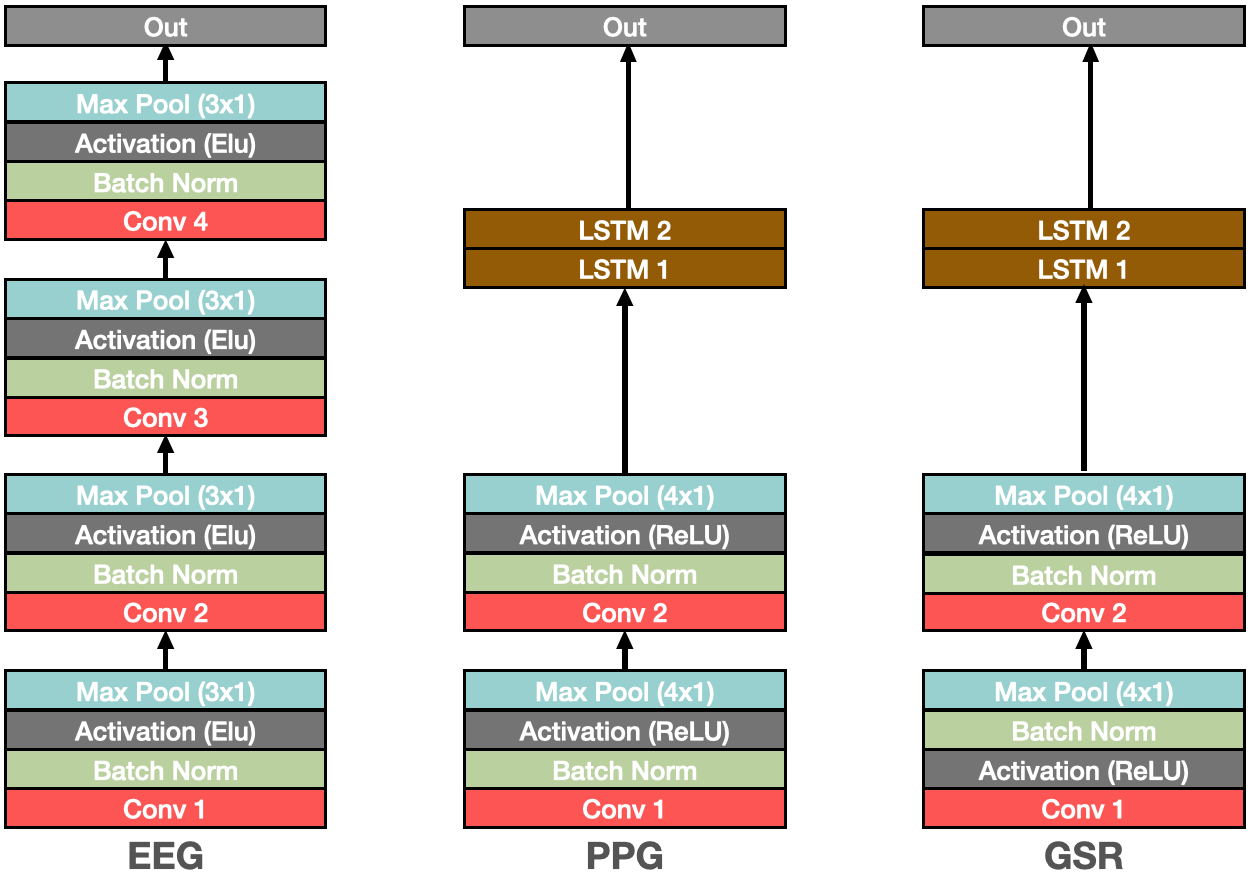
\includegraphics[scale=0.725]{single_model_architecture}
\label{fig:singlearchitecture}
\end{figure}

The utilized network for the EEG modality was a ConvNet as proposed by \citeA{schirrmeister2017deep}. The network was designed to include four convolutional blocks, each constituting a convolutional layer, followed by a batch normalization layer. The Exponential Linear Unit, hereafter referred to as "ELU", function was utilized as activation function. Each convolutional block is closed with a max pooling layer of stride three.

The utilized network for the GSR modality was a LSTM ConvNet hybrid, inspired upon by the work of \citeA{sun2019hybrid} and \citeA{dolmans2020perceived}. The network was designed to include two convolutional blocks, each constituting a convolutional layer, followed by a batch normalization layer, the activation layer and closed with a max-pooling layer of stride four. The Rectified Linear Unit, hereafter referred to as "ReLU", function was utilized as activation function. Following these two convolutional blocks are two LTSM layers.

Lastly, the utilized network for the PPG modality was inspired from the network as proposed by \citeA{biswas2019cornet}. The nework opens with two convolutional blocks, each consisting of a convolutional layer, batch normalization layer, activation layer and closed with a max pooling layer of stride four. The utilized activation function was the ReLU. Following these convolutional blocks are two LTSM layers, equal to the GSR network. 

\subsubsection{Multi-modular Network: Architecture}
The network architecture that is utilized for the multi-modular approach is determined by a combination of the single-modular networks, as derived from the literature. The previously delineated design principles (i.e. the principles of modularity and generalizability) are taken into account when doing so. The visual representation of the multi-modular network is depicted as figure \ref{fig:multiarchitecture}.

\begin{figure}
\caption{Multi-modular Network Architecture}
\bigskip
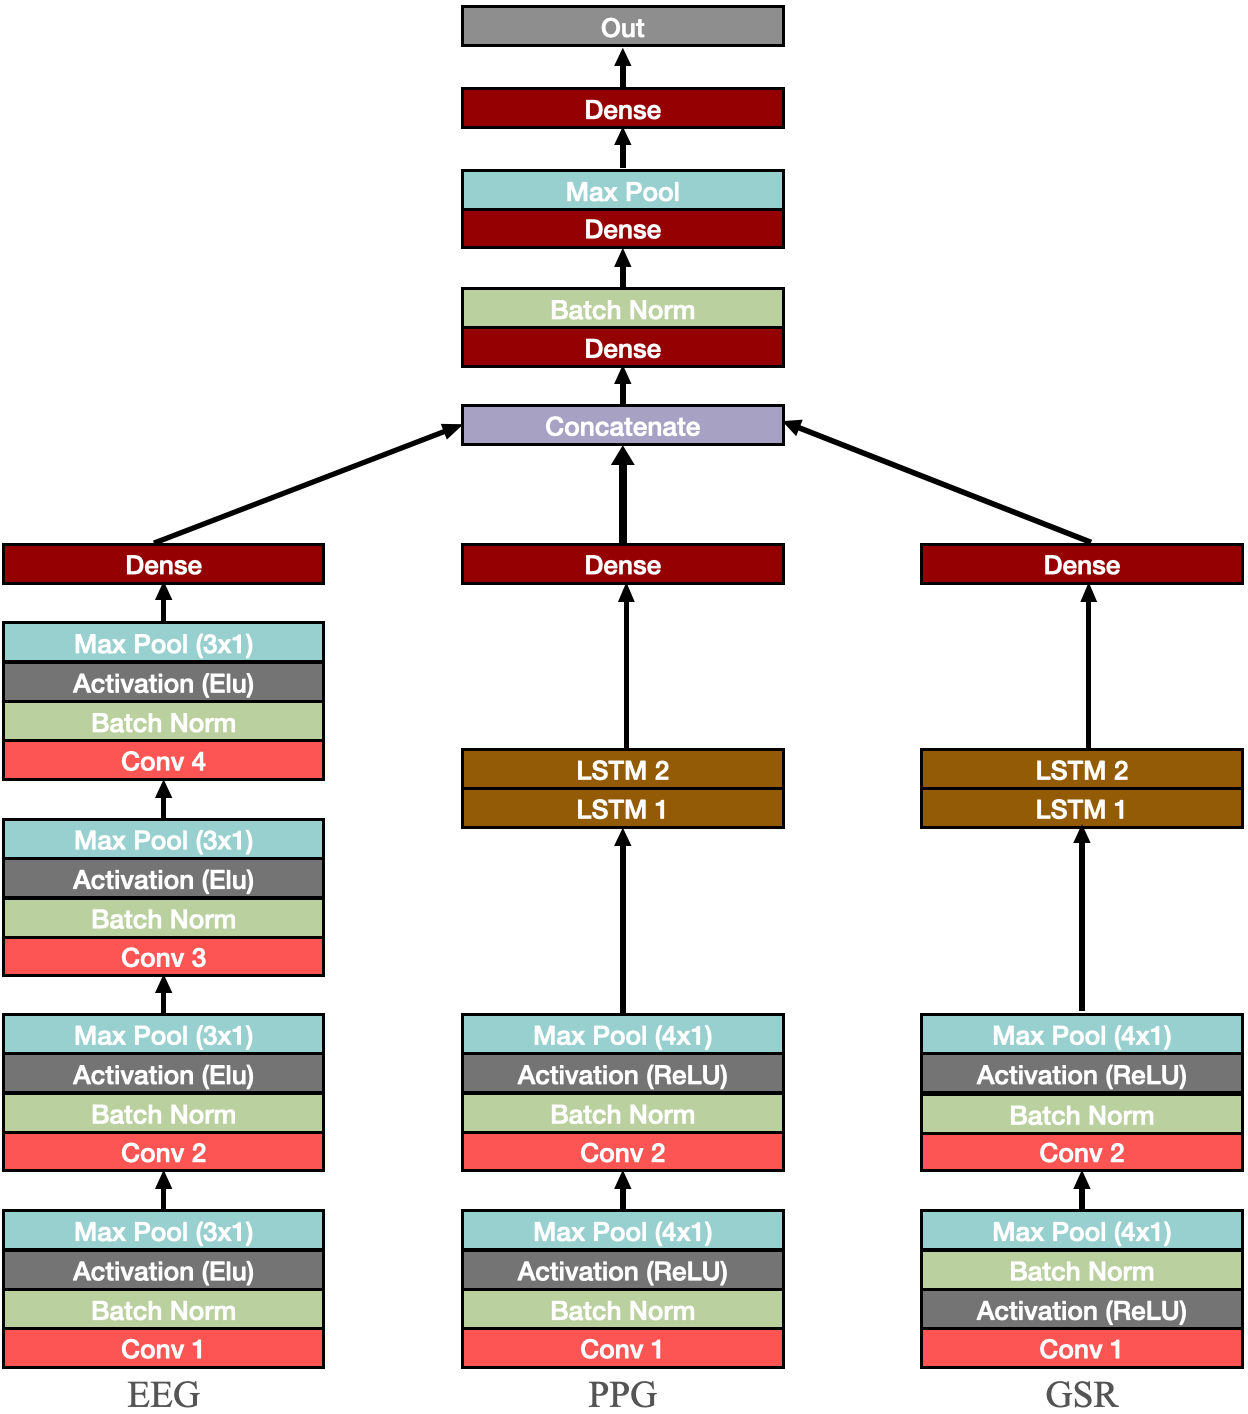
\includegraphics[scale=0.725]{multi_model_architecture}
\label{fig:multiarchitecture}
\end{figure}

In order to combine the previously delineated single-modular networks, each of these distinct parts are closed with one fully connected dense layer before feeding into the head network. This is done in order to flatten all inputs into a lower dimensional space, such that concatenation is possible. The head network consists of four dense layers. These layers are alternated with a batch normalization and max-pooling layer with the objective of stabilization. 

\subsubsection{Multi-modular Network: Variations}
Speed is a potential bottleneck for a multi-modular network that should be able to classify in real-time. The previously delineated network is substantially complex in nature. Therefore, several variations of this network have been investigated upon, each differing in their complexity. These variations are not made by altering the network architecture, for deviating from the distinguished architecture might be detrimental towards performance. The goal is to propose a network that is fast enough for real-time classification, whilst maintaining the highest amount of accuracy as possible. Three different variations with regards to size of the network as depicted in figure \ref{fig:multiarchitecture} have therefore been considered.

Network size can be understood as the amount of specified filters for convolutional layers, and the amount of specified neurons for all other utilized layers. A decrease in the amount of filters and neurons constitutes a decrease in network size, and consequently a decrease in the amount of required calculations. Doing so brings about an increase in speed. An overview of all three multi-modular network variations, and the amount of specified neurons/filters per layer, is provided in table \ref{table:modelvariations}. Network 1 is referred to as the full network, and is the biggest in terms of size. The size of network 2 constitutes of 75 \% of the size of the full network. Network 3 constitutes of 50 \% of the size of the full network.

\bgroup
\def\arraystretch{1.6}%  
\begin{table}[h]
\centering
\caption{Model variation sizes}
\label{table:modelvariations}
\begin{tabular}{lllll}
\hline
        & EEG        & GSR        & PPG        & Head       \\ \hline
Network 1 & Conv1: 25  & Conv1: 128 & Conv1: 128 & Dense: 712 \\
        & Conv2: 50  & Conv2: 128 & Conv2: 128 & Dense: 356 \\
        & Conv3: 100 & LSTM1: 256 & LSTM1: 256 & Dense: 178 \\
        & Conv4: 200 & LSTM1: 256 & LSTM2: 256 &            \\ 
        \vspace{3ex}
        & Dense: 200 & Dense: 256 & Dense: 256 &            \\ \hline
Network 2 & Conv1: 18  & Conv1: 96  & Conv1: 96  & Dense: 534 \\
        & Conv2: 34  & Conv2: 96  & Conv2: 96  & Dense: 267 \\
        & Conv3: 75  & LSTM1: 192 & LSTM1: 192 & Dense: 134 \\
        & Conv4: 150 & LSTM1: 192 & LSTM1: 192 &            \\
        \vspace{3ex}
        & Dense: 150 & Dense: 192 & Dense: 192 &            \\ \hline
Network 3 & Conv1: 13  & Conv1: 64  & Conv1: 64  & Dense: 356 \\
        & Conv2: 25  & Conv2: 64  & Conv2: 64  & Dense: 178 \\
        & Conv3: 50  & LSTM1: 128 & LSTM1: 128 & Dense: 89  \\
        & Conv4: 100 & LSTM1: 128 & LSTM2: 128 &            \\
        & Dense: 100 & Dense: 128 & Dense: 128 &            \\ \hline
\end{tabular}
\vspace{2ex}

\begin{doublespacing}
{\raggedright \textit{Note:} For all convolutional layers the depicted number reflects the amount of utilized filters, whereas for LTSM layers it reflects the amount  of nodes. \par}
\end{doublespacing}
\end{table}
\egroup

\clearpage
\subsection{Model Evaluation}
The network performances have been assessed and contrasted by means of several performance metrics. The utilized metrics constitute six well known and widely applied metrics, all constructed from the confusion matrix, depicted as table \ref{table:confusion}.

\bigskip
\bgroup
\def\arraystretch{1.6}%  
\begin{table}[h]
\centering
\caption{Confusion matrix}
\label{table:confusion}
\begin{tabular}{lll}
                                        & True Positive          & True Negative          \\ \cline{2-3} 
\multicolumn{1}{l|}{Predicted Positive} & \multicolumn{1}{l|}{a} & \multicolumn{1}{l|}{b} \\ \cline{2-3} 
\multicolumn{1}{l|}{Predicted Negative} & \multicolumn{1}{l|}{c} & \multicolumn{1}{l|}{d} \\ \cline{2-3} 
\end{tabular}
\end{table}
\egroup

The measures accuracy, sensitivity, specificity, PPV, NPV and F1 have been utilized in order to asses network performance. The network that performs best across these measures was considered to be the superior performing network. Table \ref{table:metrics} depicts the constitution of these performance metrics, by partly referring to confusion matrix depicted as table \ref{table:confusion}. 
\bigskip
\bgroup
\def\arraystretch{1.8}%  
\begin{table}[h]
\centering
\caption{Performance Metrics}
\label{table:metrics}
\begin{tabular}{ll}
\hline
Accuracy:                       & \(\frac{\!\!\!\!\!\!\!\!\!\!\!\!\!\!a+d}{a+b+c+d}\) \\
Sensitivity:                    & \(\frac{a}{a+c}\)                                   \\
Specificity:                    & \(\frac{d}{b+d}\)                                   \\
Positive Predicted Value (PPV): & \(\frac{a}{a+b}\)                                   \\
Negative Predicted Value:       & \(\frac{d}{c+d}\)                                   \\
F1-measure:                     & \(\frac{2*Sensitivity*PPV}{Sensitivity+PPV}\)       \\ \hline
\end{tabular}
\end{table}
\egroup

\newpage

\bibliographystyle{apacite}
\bibliography{References}

\end{document}
